\begin{figure}[h!t]
 \centering
 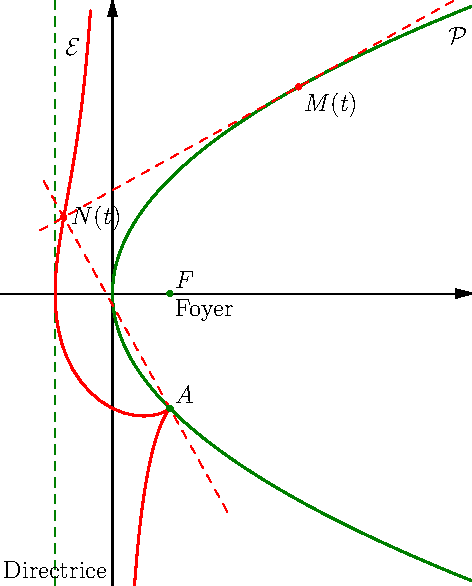
\includegraphics{./Cpapota_1.pdf}
 % Cpapota_1.pdf: 0x0 pixel, 0dpi, 0.00x0.00 cm, bb=
 \caption{Podaire d'un point de la parabole}
 \label{fig:Cpapota_1}
\end{figure}

\begin{enumerate}
 \item
\begin{enumerate}
 \item On peut factoriser $\varphi(t)$ en utilisant des coefficients indéterminés ou une division euclidienne polynomiale. On obtient
\begin{displaymath}
 \varphi(t) = (t+1)(t^3-t^2+3t+1)
\end{displaymath}

 \item Notons $\psi(t) = t^3-t^2+3t+1$. La dérivée $\psi'(t) =3t^2-2t+3$ est une fonction du second degré dont le discriminant est strictement négatif ($=-32$). Elle est à valeurs strictement positives. On en déduit que $\psi$ est strictement croissante. Comme $\psi(-1)=4$ et $\psi(0)=1$, elle s'annule en un unique réel $\alpha\in ]-1,0[$. 
\end{enumerate}
 
 \item L'axe focal de la parabole $\mathcal P$ est l'axe $Ox$ car il contient le sommet et le foyer. Le sommet d'une parabole est à égale distance du foyer et du point d'intersection de l'axe focal avec la directrice (figure \ref{fig:Cpapota_1}). On en déduit que la directrice est la droite d'équation $x=-1$. On en tire l'équation de $\mathcal{P}$ qui est
\begin{displaymath}
 y^2 = 4x
\end{displaymath}

 \item 
\begin{enumerate}
 \item Les coordonnées de $M(t)$ sont $(t^2,2t)$. En calculant la vitesse et en utilisant un déterminant, on forme l'équation de la tangente $D_t$.
\begin{displaymath}
 \begin{vmatrix}
  x-t^2 & 2t \\y-2t & 2
 \end{vmatrix}
=0
\Leftrightarrow
x-ty+t^2 = 0
\end{displaymath}

 \item Le vecteur $\overrightarrow n$ de coordonnées $(1,-t)$ est normal à $D_t$. Le projeté $N(t)$ de $A$ sur $D_t$ est de la forme $A+\lambda \overrightarrow n$. On calcule $\lambda$ en injectant dans l'équation de $D_t$ l'expression des coordonnées de $N(t)$. On trouve
\begin{displaymath}
 \lambda = -\frac{(1+t)^2}{1+t^2}
\end{displaymath}
On en déduit
\begin{displaymath}
 \text{coordonnées de }N(t):
\left(\frac{-2t}{1+t^2} ,\frac{-2+t+t^3}{1+t^2}\right) 
\end{displaymath}
\end{enumerate}

 \item
\begin{enumerate}
 \item On définit des fonctions $u$ et $v$ par $u(t)=x(N(t))$ et $v(t)=y(N(t))$. Le calcul des dérivées conduit à :
\begin{align*}
 u'(t)=2\frac{t^2-1}{(1+t^2)^2} & &
v'(t)=\frac{t^4+2t^2+4t+1}{(1+t^2)^2}=\frac{(t+1)\psi(t)}{(1+t^2)^2}
\end{align*}
On en déduit le tableau des variations.
\begin{center}
\renewcommand{\arraystretch}{1.2}
\begin{tabular}{|cccccccccccc|} \hline 
 & $-\infty$ &  & $-1$ &  & $\alpha$ &  & $0$ &  & $1$ &  & $+\infty$\\ \hline
u & $0$ & $\nearrow$ & $1$ &  & $\searrow$ &  &  &  &  & $\nearrow$  & $0$\\ \hline
$v$ & $-\infty$ & $\nearrow$ & $-2$ & $\searrow$ &  &  & $\nearrow$ &  &  &  & $+\infty$ \\ \hline
\end{tabular}
\end{center}

 \item Il existe deux branches infinies pour $t$ en $-\infty$ ou en $+\infty$. Dans chaque cas, la droite d'équation $x=0$ est asymptote.\newline
En $-\infty$, la courbe est à droite de l'asymptote. En $+\infty$, la courbe est à gauche de l'asymptote.
 \item Le point $A\in \mathcal{E}$ car comme il appartient à $\mathcal{P}$, il est son propre projeté orthogonal sur la tangente en $A$. En fait $A=M(-1)=N(-1)$.\newline
Il apparait sur le tableau de variations que $A$ est un point stationnaire car $u'(-1)=v'(-1)=0$. On peut factoriser la vitesse:
\begin{displaymath}
 \overrightarrow{N}'(t)=\frac{t+1}{(1+t^2)^2}
\left(
\underset{=\overrightarrow d(t)}{\underbrace{4(t-1)\overrightarrow i +\psi(t)\overrightarrow j}}
 \right) 
\end{displaymath}
Le choix de $\overrightarrow d (t)$ comme vecteur directeur de $D_t$ montre que la tangente en $A$ admet $\overrightarrow d(-1)$ comme vecteur directeur. La direction en $A$ est donc $\overrightarrow i + \overrightarrow j$.

\end{enumerate}

 \item 
\begin{enumerate}
 \item On se donne trois points arbitraires de coordonnées $(x_1,y_1)$, $(x_2,y_2)$, $(x_3,y_3)$ et on considère le système $\mathcal S$ aux inconnues $a$, $b$, $c$ :
\begin{displaymath}
 \mathcal{S}\hspace{0.5cm}
\left\lbrace
\begin{aligned}
x_1 a + y_1 b +c &=0 \\ 
x_2 a + y_2 b +c &=0 \\
x_3 a + y_3 b +c &=0 
\end{aligned}
\right. 
\end{displaymath}
Si les trois points sont alignés, il existe une droite d'équation $ax+by+c=0$ (avec $(a,b)\neq(0,0)$) qui les contient tous les trois. Le système admet donc une solution autre que $(0,0,0)$ et le déterminant doit être nul.\newline
Réciproquement, si le déterminant est nul, le système admet une solution $(a,b,c)\neq(0,0,0)$. En fait $(a,b)\neq(0,0)$ car $(a,b)=(0,0)$ entraine $c=0$. On peut donc considérer la droite d'équation $ax+by+c=0$, elle contient les trois points qui sont donc alignés.
 \item Le calcul se fait chaque fois en utilisant $L_3 \leftarrow L_3 - L_2$ puis $L_2 \leftarrow L_2 - L_1$ (ce qui ne change pas le déterminant). On utilise ensuite la multilinéarite.
\begin{multline*}
  \begin{vmatrix}
  1 & t_1 & t_1^2 \\ 1 & t_2 & t_2^2 \\ 1 & t_3 & t_3^2 
 \end{vmatrix}
=
  \begin{vmatrix}
  1 & t_1 & t_1^2 \\ 1 & t_2 & t_2^2 \\ 0 & t_3-t_2 & t_3^2-t_2^2 
 \end{vmatrix}
=
  \begin{vmatrix}
  1 & t_1 & t_1^2 \\ 0 & t_2-t_1 & t_2^2-t_1^2 \\ 0 & t_3-t_2 & t_3^2-t_2^2 
 \end{vmatrix} \\
= (t_2-t_1)(t_3-t_2)
  \begin{vmatrix}
  1 & t_1 & t_1^2 \\ 0 & 1 & t_2+t_1 \\ 0 & 1 & t_3+t_2 
 \end{vmatrix} \\
= (t_2-t_1)(t_3-t_2)
  \begin{vmatrix}
  1 & t_1 & t_1^2 \\ 0 & 1 & t_2+t_1 \\ 0 & 0 & t_3+t_1 
 \end{vmatrix}
= (t_2-t_1)(t_3-t_2)(t_3-t_1)
\end{multline*}

\begin{multline*}
  \begin{vmatrix}
  1 & t_1 & t_1^3 \\ 1 & t_2 & t_2^3 \\ 1 & t_3 & t_3^3 
 \end{vmatrix}
=
  \begin{vmatrix}
  1 & t_1 & t_1^3 \\ 0 & t_2-t_1 & t_2^3-t_1^3 \\ 0 & t_3-t_2 & t_3^3-t_2^3 
 \end{vmatrix}\\
= (t_2-t_1)(t_3-t_2)
  \begin{vmatrix}
  1 & t_1 & t_1^3 \\ 0 & 1 & t_2^2+t_1t_2+t_1^2 \\ 0 & 1 & t_3^2+t_2t_3+t_2^2 
 \end{vmatrix} \\
= (t_2-t_1)(t_3-t_2)\left(t_3^2-t_1^2 +t_2(t_3-t_1)\right)\\
=  (t_2-t_1)(t_3-t_2)(t_3-t_1)(t_1+t_2+t_3)
\end{multline*}
 \item D'après la question a. on peut caractériser l'alignement par la nullité d'un déterminant que l'on transforme par multilinéarité par rapport aux lignes. Finalement: $N(t_1)$, $N(t_2)$, $N(t_3)$ sont alignés si et seulement si
\begin{displaymath}
 \begin{vmatrix}
  -2t_1 & -2+t_1+t_1^3 & 1+t_1^2 \\
  -2t_2 & -2+t_2+t_2^3 & 1+t_2^2 \\
  -2t_3 & -2+t_3+t_3^3 & 1+t_3^2 \\
 \end{vmatrix}
=0
\end{displaymath}
On note respectivement $D$ et $\Delta$ les déterminants calculés en b.
On développe ce déterminant par multilinéarité par rapport aux colonnes. On obtient la somme des déterminants
\begin{displaymath}
D_1=
 \begin{vmatrix}
  -2t_1 & -2 & 1 \\
  -2t_2 & -2 & 1 \\
  -2t_3 & -2 & 1 \\
 \end{vmatrix}
=0
\end{displaymath}
\begin{displaymath}
D_2=
 \begin{vmatrix}
  -2t_1 & -2 & t_1^2 \\
  -2t_2 & -2 & t_2^2 \\
  -2t_3 & -2 & t_3^2 \\
 \end{vmatrix}
=-4 D
\end{displaymath}
\begin{displaymath}
D_3
 \begin{vmatrix}
  -2t_1 & t_1 & 1+t_1^2 \\
  -2t_2 & t_2 & 1+t_2^2 \\
  -2t_3 & t_3 & 1+t_3^2 \\
 \end{vmatrix}
=0
\end{displaymath}
\begin{displaymath}
D_4=
 \begin{vmatrix}
  -2t_1 & t_1^3 & 1 \\
  -2t_2 & t_2^3 & 1 \\
  -2t_3 & t_3^3 & 1 \\
 \end{vmatrix}
=-2\Delta
\end{displaymath}
\begin{displaymath}
D_5=
 \begin{vmatrix}
  -2t_1 & t_1^3 & t_1^2 \\
  -2t_2 & t_2^3 & t_2^2 \\
  -2t_3 & t_3^3 & t_3^2 \\
 \end{vmatrix}
=2t_1t_2t_3 D
\end{displaymath}
En simplifiant par $2D$ qui est non nul car les points sont deux à deux distincts on obtient la relation demandée.
\end{enumerate}

 \item
\begin{enumerate}
 \item Soit $t\in \R\setminus\{-1,+1\}$ fixé. Considérons un $u\neq t$ dans $\R\setminus\{-1,+1\}$. La droite $(N(t),N(u)$ coupe $\mathcal E$ en un point $N(\theta)$ où dépend de $t$ et $u$ selon la formule de la question précédente. Lorsque $u$ tend vers $t$, la direction de la droite $(N(t),N(u))$ tend vers celle de la tangente. La droite $\Delta_t$ recoupe donc $\mathcal{E}$ seulement en $N(\theta)$ avec 
\begin{displaymath}
 t^2\theta - 2t -\theta = 2 \Rightarrow
\theta = 2\frac{1+t}{t^2-1}=\frac{2}{t-1} 
\end{displaymath}
On peut remarquer qu'en $N(1)$, la tangente est verticale et ne recoupe pas la courbe.
 \item L'étude des variations des coordonnées montre que la courbe paramétrée $N$ est simple. Un point $N(t)$ est donc son propre tangentiel si et seulement si
\begin{displaymath}
 t=\frac{1}{t-1}\Leftrightarrow t^2-t-1=0\Leftrightarrow t=1\pm\sqrt{5}
\end{displaymath}
En ces points, la courbe traverse sa tangente. Il s'agit de points d'inflexions.
 \item Notons $F(t_1,t_2,t_3) = t_1t_2t_3-(t_1+t_2+t_3)-2$ et $\theta_i = \frac{2}{t_i-1}$ pour $i=1,2,3$. Exprimons $F(\theta_1,\theta_2,\theta_3)$: après réduction au même dénominateur, développement et simplification, on obtient
\begin{displaymath}
 F(\theta_1,\theta_2,\theta_3) = -\frac{2F(t_1,t_2,t_3)}{(t_1-1)(t_2-1)(t_3-1)}
\end{displaymath}
Lorsque $N(t_1)$, $N(t_2)$, $N(t_3)$ sont alignés,
\begin{displaymath}
 F(t_1,t_2,t_3)=0 \Rightarrow F(\theta_1,\theta_2,\theta_3)=0
\end{displaymath}
et les trois tangentiels sont alignés (voir fig \ref{fig:Cpapota_2}).

\begin{figure}[h!t]
 \centering
 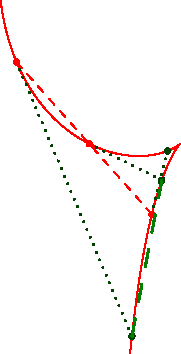
\includegraphics{./Cpapota_2.pdf}
 % Cpapota_2.pdf: 0x0 pixel, 0dpi, 0.00x0.00 cm, bb=
 \caption{Tangentiels et alignements}
 \label{fig:Cpapota_2}
\end{figure}

\end{enumerate}
\end{enumerate}
